%! Licence = CC BY-NC-SA 4.0

%! Author = gianfluetsch, mariuszindel
%! Date = 10. Jan 2021
%! Project = cydef_summary


\section{Windows Logs}

\subsection{TLP (Traffic Light Protocol)}
\begin{itemize}
    \item RED $\rightarrow$ Infos sind auf den \textbf{Kreis der Anwesenden} beschränkt $\rightarrow$ Weitergabe ist untersagt
    \item Amber $\rightarrow$ infos darf der Empfänger \textbf{innerhalb seiner Organisation} aus Basis “Kenntnis \textbf{nur wenn nötig}” weitergeben
    \item Green $\rightarrow$ infos dürfen \textbf{innerhalb der Organisation} und an deren Partner weitergegeben, aber \textbf{nicht veröffentlicht} werden
    \item White (default) $\rightarrow$ abgesehen von \textbf{urheberrechtlichen Aspekten} dürfen die Infos \textbf{ohne Einschränkungen} weitergegeben werden
\end{itemize}

\subsection{Event Log Introduction}

\subsubsection{Event Log Categories}
\begin{itemize}
    \item \textbf{Security.evtx}
    \begin{itemize}
        \item access control and seucrity information
        \item only written by \textit{LSASS} process (based on GPO Settings)
        \item \glqq Security Event Log\grqq is \textcolor{red}{most important for cyber defense}
        \item System events, logon, account, privilege used, account management, object access, directory service, process tracking
    \end{itemize}
    \item \textbf{System.evtx}
    \begin{itemize}
        \item windows system events (driver, service, ressources)
    \end{itemize}
    \item \textbf{Application.evtx}
    \begin{itemize}
        \item non system related software events
    \end{itemize}
    \item \textbf{<Custom>.evtx}
    \begin{itemize}
        \item around 150 different custom application logs
    \end{itemize}
\end{itemize}

\subsubsection{Security.evtx - Account Monitoring}
\textbf{Event IDs}
\begin{itemize}
    \item \textbf{4624} - Successful Logon
    \item \textbf{4624/ 4647/ 4634} - Successful Logoff
    \item \textbf{4625} - Failed Logon
    \item \textbf{4648} - Logon with explicit credentials
    \item \textbf{4672} - Special privileges assigned to new logon
    \item \textbf{4688} - show any processes created by anybody including malware and attackers
    \item \textbf{4720} - Account Creation
    \item \textbf{4738} - A user account was changed (permissions granted or similar)
    \item \textbf{4776} - Local account authentication (NTLM authentication)
    \item \textbf{4779} - A user disconnected a terminal server session without logging off
\end{itemize}

\subsubsection{Logon Type}
\begin{tabular}{ l | p{6cm} }
     2 & \textbf{Interactive} (logon at keyboard and screen of system) \\
     3 & \textbf{Network} (i.e. connection to shared folder on this computer from elsewhere on network) \\  
     4 & Batch (e.g. scheduled task) \\  
     5 & \textbf{Service} (Service startup) \\
     7 & Unlock (i.e. unnattended workstation with password protected screen saver) \\
     8 & NetworkCleartext: Logon with credentials sent in the clear text. Most often indicates a logon to IIS with basic authentication. \\
     9 & NewCredentials such as with RunAs or mapping a network drive with alternate credentials. ''A caller cloned its current token and specified new credentials for outbound connections. The new logon session has the same local identity, but uses different credentials for other network connections.'' \\
     10 & \textbf{RemoteInteractive} (Terminal Services, Remote Desktop or Remote Assistance) \\
     11 & CachedInteractive (logon with cached domain credentials such as when logging on to a laptop when away from the network)
\end{tabular}

\subsubsection{EventLog Size}
\begin{itemize}
    \item Every Event Log has a maximum size (default 20Mb)
    \item Empfohlen: Security-Log auf 4-8 GB vergrössern $\rightarrow$ ist bei Security Incidents das wichtigste Log!
    \item Three Options when the maximum size is reached
    \begin{enumerate}
        \item Overwrite events as needed $\rightarrow$ Starts rotating events out
        \item Archive the log when full $\rightarrow$ Creates Files like “Archive-Security-<Date>.evtx
        \item Do not overwrite events $\rightarrow$ Error Message is generated upon full log
    \end{enumerate}
\end{itemize}

\subsubsection{LSASS Process}
Local Security Authority Subsystem Service (LSASS) ist ein Prozess in Microsoft Windows-Betriebssystemen, der für die Durchsetzung der Sicherheitsrichtlinien auf dem System verantwortlich ist. 
Er überprüft Benutzer, die sich bei einem Windows-Computer oder -Server anmelden, bearbeitet Kennwortänderungen und erstellt Zugriffstoken.\\

\textit{lsass.exe} ist ein Windows-Prozess, der sich um die Sicherheitsrichtlinien des Betriebssystems kümmert. 
Wenn sich zum Beispiel jemand bei einem Windows-Client oder -Server anmeldet, überprüft \textit{lsass.exe} den Benutzernamen und das Kennwort. 
Wenn \textit{lsass.exe} beendet wird, wird der Benutzer von Windows abgemeldet.
\textit{lsass.exe} schreibt auch in das Windows Security-Log, so dass dort nach fehlgeschlagenen Authentifizierungsversuchen und anderen Sicherheitsrichtlinienproblemen gesucht werden kann.

\subsection{Malicious Activity Detection}

\subsubsection{Clearing (Deleting) Event Logs}
\begin{itemize}
    \item Usually results in an event \textbf{1102}
    \item \textit{Note}: There are tools that allow event log editing without an event showing (Mimikatz, etc.)
\end{itemize}

\subsubsection{Logon Status and Sub Status Codes}
\begin{tabular}{ l | p{4.5cm} }
    0xC0000064 & \textbf{user name does not exist} \\
    0xC000006A & \textbf{user name is correct but the password is wrong} \\  
    0xC0000234 & user is currently locked out \\  
    0xC0000072 & account is currently disabled \\
    0xC000006F & \textbf{user tried to logon outside his day of week or time of day rextriction} \\
    0xC0000070 & \textbf{workstation restriction or Authentication Policy Silo violation} (look for event ID 4820 on DC) \\
    0xC0000193 & account expiration \\
    0xC0000071 & expired password \\
    0xC0000133 & clocks between DC and other computer too far out of sync \\
    0xC0000224 & user is required to change password at next logon \\
    0xC0000225 & evidently a bug in Windows and not a risk \\
    0xc000015b & The user has not been granted the requested logon type (aka logon right) at this machine
\end{tabular}

\subsection{Logging}
Über eine GPO kann ein Logging-Agent (z.B. der Wazuh-Agent) einfach auf allen gewünschten Servern installiert und konfiguriert werden. Diesen Agent sollte man so konfigurieren, dass er alle wichtigen und relevanten Logs (z.B. die RDP Logs) ebenfalls an Wazuh weiterleitet. Danach sind diese Logs auch innerhalb von Wazuh zentral ersichtlich und filterbar.

Dabei werden die Events aus dem EventLog an Wazu weitergeleitet und es kann somit auch nach der \textit{EventID} gefiltert werden.

\subparagraph{Windows Logs}

\subsubsection{RDP event ID's in domain controller event log?}
Die Logs befinden sich je auf dem RDP Server unter TerminalServices-LocalSessionManager.
Diese Logs werden aktuell jedoch vom Wazuh Agent (noch) nicht an Wazuh geleitet. Daher erscheinen diese auch nicht in Wazuh. 

\subsubsection{RDP event ID's in Wazuh?}
Yes, the Wazuh agents did report/log the RDP event IDs. The event were shown on the Wazuh Web Dashboard.

\columnbreak

\subsubsection{EventID 1149}
Successful network authentication (successfully executed an RDP network connection).

Event 1149 is logged when there is a successful RDP logon to the computer. Before Windows 7 and Windows Server 2012, 1149 would be logged for any initiation of an RDP connection, so it was not a useful indicator for an actual successful application of user credentials.

But, that has changed, and all modern OS versions will only log 1149 if the username in the event was successfully authenticated. It also includes the IP address of the source of the connection, which is useful information. If an account is used and successfully authenticates but does not have permission to RDP to the computer due to other restrictions, event 1149 is not generated.

\subsubsection{Phases of RDP-Connection}
\begin{enumerate}
    \item Connection Initiation
    \item Basic Settings Exchange
    \item Channel Connection
    \item RDP Security Commencement
    \item Secure Settings Exchange
    \item Optional Connect-Time Auto-Detection
    \item Licensing
    \item Optional Multitransport Bootstrapping
    \item Capabilities Exchange
    \item Connection Finalization
\end{enumerate}
\begin{center}
    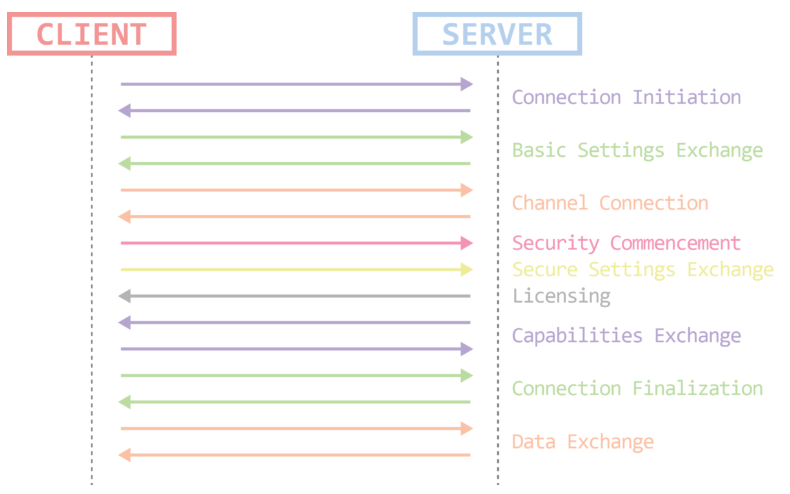
\includegraphics[width=1.0\linewidth]{./img/04-windows_logs/rdp_phases}
     \vspace{-8pt}
\end{center}

\subsubsection{Explain how you filtered every RDP login attempt}
The TerminalServices-RemoteConnectionManager Log is not forwarded to Wazuh.\\
Unable to filter for all the attempts. With the current Wazu setup, one must filter for Logon Type 3 \& 10 (remote logon types)\\

\begin{itemize}
    \item \lstinline|data.win.system.eventID = 4624| or \lstinline|data.win.system.eventID = 4625|
    \item \lstinline|data.win.sytem.eventID: 4624| and \lstinline|data.win.evendata.logonType: 3|
\end{itemize}

\subsubsection{Explain how you filtered unsuccessful RDP login attempts}
Um erfolglose RDP Login Versuche im Event Viewer zu suchen, sucht man nach der \lstinline|Event ID: 4625|.\\

\begin{itemize}
    \item \lstinline|data.win.eventdata.logonType = 3| or \lstinline|data.win.eventdata.logonType = 10|
    \item \lstinline|data.win.system.eventID = 4625| and \lstinline|data.win.eventdata.logonType = 3|
\end{itemize}

\subparagraph{Wazuh}

\subsubsection{Wazuh Agent}
The \textit{Wazuh agent} runs on monitored systems and is responsible for collecting log and event data, performing policy monitoring scans, detecting malware and rootkits and triggering alerts when monitored files are modified. It communicates with the Wazuh server through an encrypted and authenticated channel.

\subsubsection{Wazuh Manager}
\textit{Wazuh Manager} is the management console for Wazuh. It provides a UI for the collected data from Elasticsearch and Kibana.

\subsubsection{Does Wazuh agent forward plain logs from host it runs or the built-in Windows Events if agents installed on Windows computer}
Yes, the \textit{Wazuh agent} is forwarding both types of log files. The agent can e.g. collect logs from Windows EventViewer and additional special software and forward them accordingly.

\subsubsection{Wazuh Filters}
\textit{Wazuh Filters} can be used to filter the collected (already existing) logs from Elasticsearch to show only the needed and relevant logs. Since Elasticsearch indexes a lot of data, it quickly becomes confusing without filters.
In contrast, \textit{Wazuh Rules} can be applied to new (incoming) logs and generate an alarm, for example.


\subsubsection{Wazuh server}
The Wazuh server is based on a suite of applications where each application or component is designed to accomplish a certain task. These components work together to:
\begin{itemize}
    \item analyze data received from various logs,
    \item trigger alerts when a log event matches a rule,
    \item register new clients/agents, and
    \item send data to the Elastic Stack server.
\end{itemize}


\textbf{Components:}
\begin{itemize}
    \item The Wazuh manager receives and analyzes data from the agents using decoders and rules that have been created to trigger security alerts. The manager is also used to distribute configuration files to the agents, to monitor their status and to send control messages to trigger automatic actions at the agent level.
    \item The Registration Service uses a secure mechanism to register agents without any intervention from the server side.
    \item The RESTful API provides an interface to manage and monitor the configuration of the manager and agents. It is used to register agents, inspect the manager log messages, decoders and rules and provide useful information related to the agents, including their status, operating system details, and alerts related to file integrity monitoring and rootchecks.
    \item Filebeat is used to forward alerts data from Wazuh manager to Elasticsearch. This component has its own documentation developed by Elastic.
\end{itemize}